\section{Hardware Architecture}

The formulation of HFBS allows for fast bilateral solving on high\hyp{}performance CPUs or GPUs, but the resulting power consumption may prove prohibitively costly for a full system.
FPGA platforms, on the other hand, can demonstrate fast performance with better power efficiency.
This makes them a more suitable target for a system requiring multiple high\hyp{}performance processors in a single chassis that can support processing 16-camera outputs simultaneously.
To demonstrate power and performance efficiency on FPGAs, we co-designed our hardware implementation with the HFBS algorithm.
In addition to the algorithmic optimizations, we apply hardware-specific techniques such as customized variable bitwidths and bilateral-space memory partitioning to enable better performance.

We first discuss the hardware system at a high level, and then our specific design exploration for bitwidth precision and bilateral grid memory layout.
Finally, we describe the hardware-software interface of our design and how we integrate the accelerator into an application.


\subsection{Microarchitectural Design}

We focus on executing the inner loop of Algorithm~\ref{alg:heavy} with custom hardware, and maintaining the higher-level control flow in software.
In this scheme, a software application splats the optimization problem defined in Section~\ref{sec:solver} onto a bilateral grid, and transfers it to the accelerator for iterative solving.
Figure~\ref{fig:sys-overview} shows a high-level overview of how application functionality is distributed across the system.
The figure also illustrates details of our design's microarchitecture.

\begin{figure}
\centering
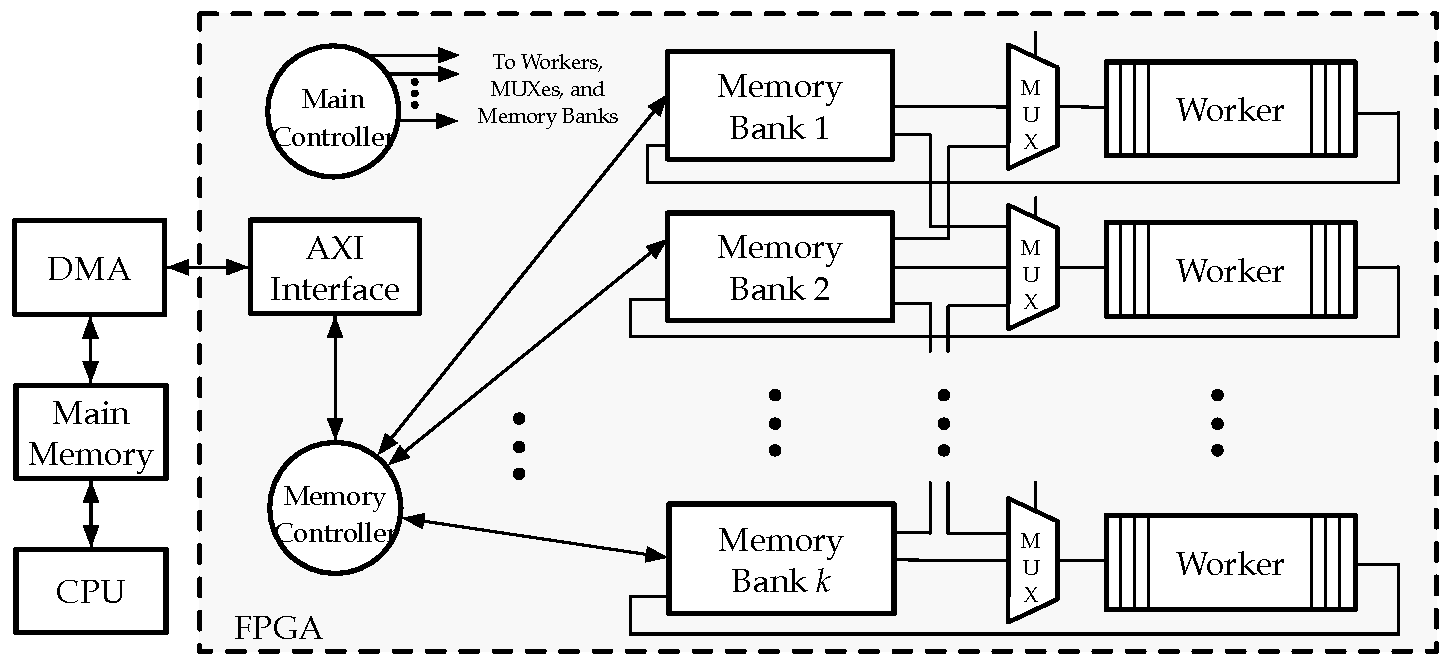
\includegraphics[width=\textwidth]{hfbs-figs/system_architecture.pdf}

\caption{High-level system overview of our accelerator. Parallel workers process bilateral grid vertices stored in partitioned memory banks.
Neighboring bank access is controlled with MUXes.
}
\label{fig:sys-overview}

\end{figure}


\paragraph{Data transfer process. }The CPU constructs the bilateral grid based on the input reference image and the initial low-resolution solution provided from prior steps.
This data is splatted onto the grid and transferred to the accelerator via direct memory access (DMA).
The transferred data includes $\hat{\mathbf{b}}$, $\mathbf{q}$, and the initial solution $\mathbf{z}_{\mathrm{init}}$ shown in Algorithm~\ref{alg:heavy}.

\begin{figure}
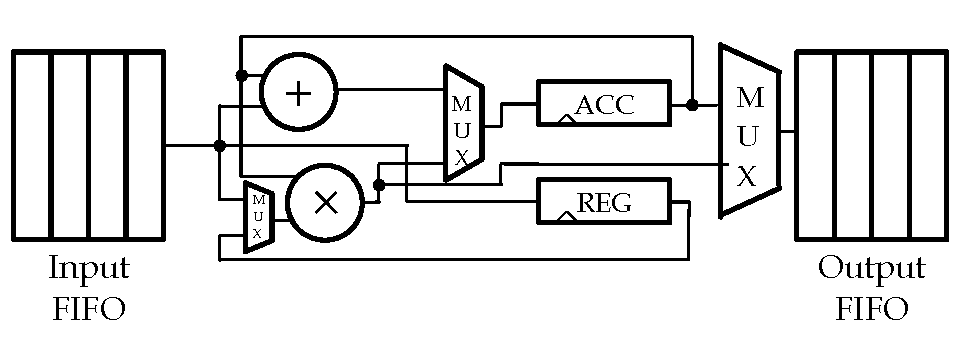
\includegraphics[width=.75\columnwidth]{hfbs-figs/worker_microarchitecture.pdf}

\caption{Block diagram of a single worker in our design.
Each worker receives the data for a grid vertex's stencil computation through an input FIFO, processes the grid vertex, and then sends the result out through an output FIFO.
}
\label{fig:microarch-single-worker}

\end{figure}

First-in-first-out queues (FIFOs) buffer data transfers at the input and output of the accelerator.
During transfer, the memory controller of Figure~\ref{fig:sys-overview} interleaves the data corresponding to each bilateral grid vertex, and partitions the data into memory banks.
After the data transfer is complete, a pool of parallel workers iteratively solve the optimization problem by running the loop of Algorithm~\ref{alg:heavy}.
Multiple grid vertices are processed in parallel and the results are updated in place.
After some number of iterations (we chose 256 iterations for our experiments to ensure convergence), the CPU reads back the final solution and slices it into a 2D result.


Each worker (shown in in Figure~\ref{fig:microarch-single-worker}) performs the inner loop of Algorithm~\ref{alg:heavy} on one grid cell.
It computes the result by streaming in the data from the neighboring cells (required for the ``blur'' operation), as well as the normalization factors required for the optimization process.
For each grid cell, a total of 6 add/subtract operations and 3 multiplications are performed. The updated result is written back to the memory.
The workers compute their local stencil operations synchronously, interfacing primarily with an assigned memory bank and occasionally the neighboring memory banks to access grid blocks that may be stored across banks.
Because each worker executes in lockstep, there are no memory collisions when accessing data in other banks.
Figure~\ref{fig:sys-overview} demonstrates how multiplexers, managed by the main controller, shepherd access to neighboring banks.
As we scale the number of workers, we find that parallelism introduces a 1\% reduction in speedup against perfect linear scaling.
This near-linear scaling can entirely be attributed to our inclusion of the ``Heavy Ball'' algorithm in HFBS, which allowed our design to use only local-neighbor communication rather than global synchronization after each iteration.


Ideally, we want the memory to be partitioned along one grid dimension only, to simplify the neighbor connections between the workers (i.e., simplify the MUXes in Figure~\ref{fig:sys-overview}).
However, this limits the number of parallel workers, to the number of grid blocks along the selected dimension.
If more parallel workers are necessary, the memory should be partition along multiple dimensions, leading to a more complicated neighbor connections.



\paragraph{Number of workers}
The number of workers is affected by several parameters such as run time requirements, power budget, and available resources. Figure~\ref{fig:worker-perf} shows how performance scales with the number of workers. Assuming we want the fastest design and have not power constraint, the number of workers will be determined by the available FPGA resources including digital signal processing units (DSPs), look-up tables (LUTs), and memory banks.

\begin{figure}
\centering
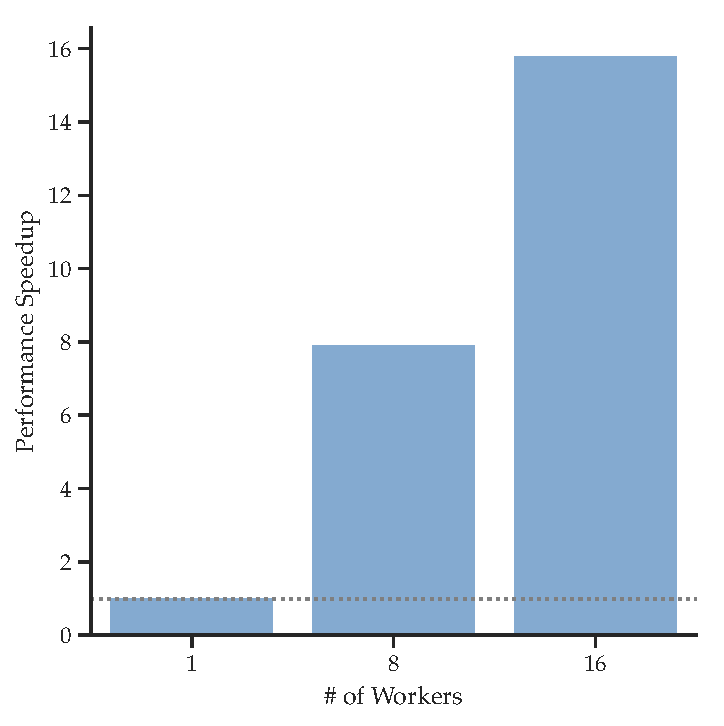
\includegraphics[width=\columnwidth]{hfbs-figs/worker_scaling.pdf}
\caption{Performance scales almost linearly with increased numbers of workers.}
\label{fig:worker-perf}
\end{figure}



\paragraph{Fixed-point Conversion} To improve resource utilization, we converted the algorithm from floating-point to fixed-point number representation.
We first implemented our workers using single-precision floating-point, like our CPU and GPU implementations.
We found that the large number of digital signal processing units (DSPs) required for a single floating-point multiplier prohibitively limited the number of workers we could employ, and consequently, the amount of parallelism.
Converting FPGA designs from floating-point to fixed-point number representation resolves this by reducing the resource requirements of hardware multipliers.
Using the cheaper fixed-point multiplier, however, required us to evaluate three competing tradeoffs: (1) the bitwidth of our fixed-point numbers, (2) the precision at a given bitwidth for the integer and fractional portions of the number, and (3) convergence of the solver.
If less than $12$ bits were used for the integer portion, the bilateral grid data would quickly populate with overflow values.
If less than $24$ bits were used for the fractional component of the number, the bilateral solver would not converge, because grid vertices would not have enough precision to capture the change in a value after blurring.

\begin{figure}
  \centering
  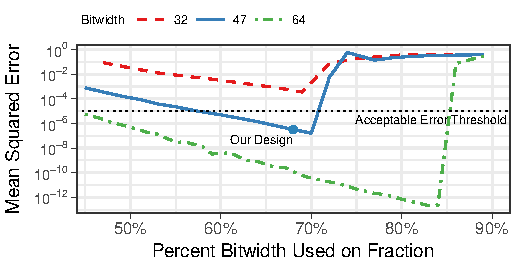
\includegraphics[width=\columnwidth]{hfbs-figs/fixed_point.pdf}
  \caption{MSE of fixed-point implementations at varied fractional widths, for different bitwidths. MSE is reported relative to 32-bit floating-point. We chose a configuration with 31 bits of fractional precision to reduce chance of overflow in the integer portion.}
  \label{fig:fixed-point}
\end{figure}

These constraints prevented us from using 32-bit fixed-point numbers, as highlighted by the high mean squared error (MSE) shown in Figure~\ref{fig:fixed-point} across integer-fraction-ratio configurations.
We delineate a maximum error threshold of $\sim 0.00001$, because any errors exceeding that precision eliminate the positive benefits of using an $\epsilon$-value to reduce zero-propagation.
Qualitatively, we also observed that a low MSE correlated with visually similar solver output that converged at the same rate as a 32-bit floating-point solver.
Using 64-bit fixed-point numbers resulted in very low MSE, but, as seen in Table~\ref{table:dsp-workers}, required 16 DSPs per worker, limiting the number of parallel workers we could deploy with these configurations.


\begin{table}[h]
  \centering
  \caption{Worker resource utilization and maximum workers at varied bitwidths. Reported MSE is relative to 32-bit floating-point.}

  \begin{tabular}{l|lll}
  \toprule
  Bitwidth        & 32                   & 47                    & 64                   \\ \midrule
  DSPs per Worker & 1                    & 4                     & 16                   \\
  Maximum Workers & 6840                  & 1710                    & 427                   \\
  Min. MSE        & $8.30\times 10^{-4}$ &  $6.69\times 10^{-7}$  & $7.16\times 10^{-13}$ \\ \bottomrule
  \end{tabular}
  \label{table:dsp-workers}


\end{table}


As a compromise, we evaluated a 47-bit number representation that was more accurate than 32-bit fixed-point, with 75\% less DSPs than 64-bit fixed-point.
To maintain some precision of 64-bit numbers during non-multiplier arithmetic, we chose a 64-bit fixed-point representation with 15 bits of integer precision and 48 bits of fractional precision, and cast it to and from 47-bit for multiply operations only.
Before multiplying two 64-bit numbers, we round off the bottom 16-bits of each number, resulting in the 1-bit sign, 15-bit integer, 31-bit fraction number highlighted in Figure~\ref{fig:fixed-point}.
We zero-extend the resulting 47-bit output back to a 64-bit number for the rest of the computation.
This fixed-point configuration has a MSE of $3.17\times10^{-7}$ compared to the floating-point implementation, resulting in negligible accuracy loss at the solver output, and the solver converges at the same number of iterations.


\subsection{Bilateral Grid Storage and Memory Layout}

\paragraph{Grid storage size's impact on quality.} Instead of a simple filter like moving average, BSSA maps a noisy depth map to a bilateral grid, refines the depth map by solving an optimization problem, and remaps the bilateral-grid result to pixel-space. Varying the number of pixels that map to a grid vertex impacts the time to compute the stereo refinement for a frame, and also the quality of the depth map. Figure~\ref{fig:vr-res-qual} demonstrates the tradeoff between stereo image quality and bilateral grid size to be processed for high-resolution input images.

\begin{figure}[h]
\centering
    \begin{center}
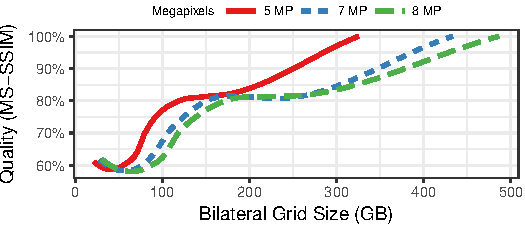
\includegraphics[width=.45\textwidth]{nsp-figs/vr_res_qual.pdf}
    \end{center}
    \caption{Using a smaller bilateral grid is cheaper to compute but degrades the quality of the output depth map, even at high image resolutions. }
    \label{fig:vr-res-qual}
\end{figure}

Here, we scaled bilateral grid sizes from 4 pixels-per-grid-vertex to 64 in each of three dimensions in a bilateral grid and evaluated the resulting impact on quality using MS-SSIM~\cite{msssim}. We find the resolution of the input images is less impactful than choosing an appropriate grid size to balance quality and computational complexity.

\paragraph{On-chip memory layout.}
To take advantage of block RAM distribution on the FPGA, we partitioned the bilateral grid into chunks along different dimensions, and dedicated grid workers for each partition.
For large, finely divided grids with many vertices (the largest grids we consider have up to 5 million vertices), we could achieve full resource utilization simply by partitioning the grid along one dimension and allocating a single worker to process each memory bank.
For more coarse grids, we partitioned the memory in multiple dimensions.

Our method for laying out data in memory consists of storing all the data needed for a grid vertex in a single packet, and writing the packets sequentially in memory.
Rather than storing multiple bilateral grid data structures separately and repeatedly indexing into each of them to process a single vertex, we interleave the data structures together to access all the information for processing a grid vertex as a single packet.
When a worker is assigned a grid vertex to process, it can fetch most of the data required for its computation from a single partition, including neighboring vertex data for some dimensions.
For large grids, where we only partition on one dimension, the data for two of the three dimensions is stored in the same memory bank, and the worker only has to communicate across banks for the two neighbors in other partitions.
For smaller grids, where we partition along multiple dimensions to improve parallelism, workers may need to fetch more of their neighbors from neighboring partitions.
All inter-bank communication is handled via the main controller of Figure~\ref{fig:sys-overview}.

To aid in fetching grid vertex data for a worker's vertex or neighboring ones, we abstracted this memory layout into a simple addressing method: we dedicate $\lceil\log_2(k)\rceil$ bits of address space for each grid dimension with size  $k$, and use the last three bits to index into the packet for a grid vertex.
For instance, with a bilateral grid of shape $\big[ 247, 166, 16\big]$ partitioned on the first dimension only, a worker assigned the address \texttt{0b 00001010 10100001 0100 001} would map the first dimension's value to memory bank $10$, and use the second and third dimensions to fetch the second item in the packet for grid vertex $\big[ 10, 161, 4\big]$.
Indexing into a neighboring vertex in any dimension means incrementing or decrementing a dimension's tag; the main controller detects when a worker is requesting an address in a neighboring bank and multiplexes the request appropriately.
This discrete mapping of grid dimensions to address spaces results in simple logic for memory addressing, but at the cost of wasted memory space.
Each grid vertex packet contains five items but requires the memory space for eight.
The same is true at the grid partition level, since the number of grid vertices along a dimension is a function of the image resolution and the $\sigma_{xy}$ or $\sigma_{l}$, and does not often fit nicely in power-of-two partitions.



\subsection{FPGA Implementation}

To invoke the bilateral solver accelerator in an application, the application sends a bytestream of bilateral grid data over the FPGA's PCIe-to-AXI DMA interface.
Once the accelerator finishes processing the bilateral grid, it sends the data back in a bytestream to the program over the same interface.
The FPGA's driver can be invoked with standard Unix I/O system calls like $read()$ and $write()$, and can thus be integrated with software applications written in any high-level language.

Some parameters of our design are fixed at configuration time, while others can be modified by software.
At configuration time, we fix the number of grid workers, memory size, and partitioning based on a chosen set of parameters for image resolution and bandwidths in the luma and spatial dimensions.
The parameters essentially define the maximum memory size and number of partitions, which can be interpreted as the upper bound of grid sizes that can be run under a certain configuration.
The bilateral grid dimensions and number of iterations are software-defined at program runtime.
Before an application sends a bilateral grid to the accelerator for processing, it first sends these software-defined parameters.
If the program requests to process a grid too large for the FPGA's configuration, the accelerator will return an error.
This level of flexibility in our design allows applications to process images of varied resolutions at varied grid bandwidths, but can result in wasted resources if the grid size being processed is much smaller than the accelerator's configured grid size.
